\documentclass[12pt]{article}
\usepackage[paper=letterpaper,margin=1.5cm]{geometry}
\usepackage{amsmath}
\usepackage{amssymb}
\usepackage{amsfonts}
\usepackage{newtxtext, newtxmath}
\usepackage{enumitem}
\usepackage{titling}
\usepackage{svg}
\usepackage{xcolor}
\usepackage{listings}
\usepackage{float}
\usepackage{nicefrac}
\usepackage[most]{tcolorbox}
\usepackage[colorlinks=true]{hyperref}

\setlength{\droptitle}{-6em}

\definecolor{codegreen}{rgb}{0,0.6,0}
\definecolor{codegray}{rgb}{0.5,0.5,0.5}
\definecolor{codepurple}{rgb}{0.58,0,0.82}
\definecolor{backcolour}{rgb}{0.95,0.95,0.92}
\definecolor{bg}{rgb}{1,0.96,0.9}

\lstdefinestyle{mystyle}{
  commentstyle=\color{codegreen},
  keywordstyle=\color{magenta},
  numberstyle=\tiny\color{codegray},
  stringstyle=\color{codepurple},
  basicstyle=\ttfamily\footnotesize,
  breakatwhitespace=false,
  breaklines=true,
  captionpos=b,
  keepspaces=true,
  numbers=left,
  numbersep=5pt,
  showspaces=false,
  showstringspaces=false,
  showtabs=false,
  tabsize=2
}

% \tcbset{enlarge left by=-0.8cm,left=1.2cm,enlarge right by=-2cm,right=0.8cm}

\lstset{
  style=mystyle,
  inputencoding=utf8,
  extendedchars=true,
}

\begin{document}

\textit{Note: intermediate steps were calculated using \texttt{numpy} and, in general, will not be shown.}

\begin{enumerate}[leftmargin=\labelsep]
  \begin{tcolorbox}[enhanced jigsaw,colback=bg,boxrule=0pt,arc=1pt,halign=center]
    \item Consider a network with three layers: 5 inputs, 3 hidden units and 2 outputs
    where all units use a sigmoid activation function.

    \begin{enumerate}
      \item {Initialize connection weights to 0.1 and biases to 0. Using the squared
            error loss, do a stochastic gradient descent update (with learning rate $\eta = 1$)
            for the following training example:

            \begin{equation*}
              x = \begin{bmatrix}
  1 & 1 & 0 & 0 & 0\\
\end{bmatrix}^T, \quad z = \begin{bmatrix}
  1 & 0\\
\end{bmatrix}^T
            \end{equation*}} \label{ex-1-a}

      \item {Compute the MLP class for the query point $x_{new} = \begin{bmatrix}
  1\\
  2\\
  3\\
\end{bmatrix}^T$} \label{ex-1-b}
    \end{enumerate}
  \end{tcolorbox}

  \textit{As an initial note, the \textit{input amount} in the input layer matches each sample's
    feature count, \underline{not} the amount of training samples.}

  The Multi-Layer Perceptron (MLP) is a feed-forward neural network with one or more hidden layers
  between the input and output layers. To train an MLP, we need to define a loss function and
  optimize it using gradient descent. The loss function is a measure of how well the network
  performs on the training data. The goal is to minimize the loss function by adjusting the
  weights and biases of the network. Our training will go through a number of epochs, each
  one with three main phases:

  \begin{enumerate}
    \item \textbf{Forward pass}: compute the output of the network for a given input
    \item \textbf{Backward pass}: compute the gradient of the loss function with respect to the
          weights and biases
    \item \textbf{Update}: update the weights and biases using the gradient
  \end{enumerate}

  The question's statement gives us, for starters, the initial weights and biases
  for the network. Note that each weight matrix has $j$ columns, one for each neuron
  in layer $\ell$, and $i$ lines, one for each neuron in layer $\ell + $. Each
  bias matrix has only one column, with $i$ lines, here following the same logic
  as the one for the weight matrices.

  \begin{equation*}
    w_1 = \begin{bmatrix}
  0.1 & 0.1 & 0.1 & 0.1\\
  0.1 & 0.1 & 0.1 & 0.1\\
  0.1 & 0.1 & 0.1 & 0.1\\
  0.1 & 0.1 & 0.1 & 0.1\\
\end{bmatrix}, \quad
    w_2 = \begin{bmatrix}
  -0.926984\\
  -2.90718\\
  -4.91178\\
\end{bmatrix}, \quad
    b_1 = \begin{bmatrix}
  0\\
  0\\
  0\\
  0\\
\end{bmatrix}, \quad
    b_2 = \begin{bmatrix}
  0.1\\
  0.1\\
  0.1\\
\end{bmatrix}
  \end{equation*}

  As we know, the forward propagation's successive \textbf{net} ($z$) and \textbf{layer output} $x$
  values are given by:

  \begin{equation*}
    \begin{aligned}
      z^{[\ell]} = w^{[\ell]} x^{[\ell-1]} + b^{[\ell]}, \quad
      x^{[\ell]} = f(z^{[\ell]})
    \end{aligned}
  \end{equation*}

  Here, of course, as stated in the question, we have $f(z) = \sigma(z)$, where $\sigma(z)$ is the
  sigmoid function. Let's start to propagate forwards:

  \begin{equation*}
    z^{[1]} = w^{[1]} x^{[0]} + b^{[1]}
    = \begin{bmatrix}
  0.1 & 0.1 & 0.1 & 0.1\\
  0.1 & 0.1 & 0.1 & 0.1\\
  0.1 & 0.1 & 0.1 & 0.1\\
  0.1 & 0.1 & 0.1 & 0.1\\
\end{bmatrix} \begin{bmatrix}
  1\\
  1\\
  0\\
  0\\
  0\\
\end{bmatrix} + \begin{bmatrix}
  0\\
  0\\
  0\\
  0\\
\end{bmatrix}
    = \begin{bmatrix}
  0.2 & 1\\
  0.2 & 1\\
  0.2 & 1\\
  0.2 & 1\\
\end{bmatrix}
  \end{equation*}

  \begin{equation*}
    x^{[1]} = f(z^{[1]}) = \sigma(z^{[1]}) = \begin{bmatrix}
  1 & 0 & 0 & 0\\
\end{bmatrix}
  \end{equation*}

  In a similar manner, we're also able to calculate both the net and the output
  of the second layer:

  \begin{equation*}
    z^{[2]} = \begin{bmatrix}
  0.216525 & 0.4202\\
  0.216525 & 0.4202\\
  0.216525 & 0.4202\\
\end{bmatrix}, \quad x^{[2]} = \begin{bmatrix}
  0\\
  1\\
\end{bmatrix}
  \end{equation*}

  Regarding the back pass, we need to compute the gradient of the loss function with respect to
  the weights and biases. The loss function is the squared error loss, which is given by
  $E = \frac{1}{2} \sum_{i=1}^n (x_i - z_i)^2$.
  The gradient of the loss function with respect to the weights and biases is given by:

  \begin{equation*}
    \frac{\partial E}{\partial w^{[\ell]}} = \textcolor{teal}{\frac{\partial E}{\partial z^{[\ell]}}} \frac{\partial z^{[\ell]}}{\partial w^{[\ell]}} = \textcolor{teal}{\frac{\partial E}{\partial z^{[\ell]}}} (x^{[\ell-1]})^T, \quad
    \frac{\partial E}{\partial b^{[\ell]}} = \textcolor{teal}{\frac{\partial E}{\partial z^{[\ell]}}} \frac{\partial z^{[\ell]}}{\partial b^{[\ell]}} = \textcolor{teal}{\frac{\partial E}{\partial z^{[\ell]}}}
  \end{equation*}

  \begin{equation*}
    \frac{\partial z^{[\ell]}}{\partial w^{[\ell]}} = (x^{[l-1]})^T, \quad
    \frac{\partial z^{[\ell]}}{\partial b^{[\ell]}} = 1
  \end{equation*}

  Considering $L$ as the last (output) layer:

  \begin{equation*}
    \delta^{[L]} = \textcolor{teal}{\frac{\partial E}{\partial z^{[L]}}}
    = \textcolor{teal}{\frac{\partial E}{\partial x^{[L]}}} \circ \frac{\partial x^{[L]}}{\partial z^{[L]}}
    = \textcolor{teal}{\frac{\partial E}{\partial x^{[L]}}} \circ f'(z^{[L]})
    = (x^{[L]} - z) \circ \sigma(z^{[L]}) \circ (1 - \sigma(z^{[L]}))
  \end{equation*}

  \begin{equation*}
    \underset{l \neq L}{\delta^{[\ell]}} = \textcolor{teal}{\frac{\partial E}{\partial z^{[\ell]}}}
    = (\frac{\partial z^{[\ell+1]}}{\partial x^{[\ell]}})^T \delta^{[\ell+1]} \circ f'(z^{[\ell]})
    = (w^{[\ell+1]})^T \delta^{[\ell+1]} \circ \sigma(z^{[\ell]}) \circ (1 - \sigma(z^{[\ell]}))
  \end{equation*}

  Note that the sigmoid function's derivative is a well known derivative,
  which you should know (or bring in your note sheet). Moreover, the error's
  derivative regarding $x^{[L]}$ is represented here without the $\Sigma$ sign,
  since we're dealing with a single training example.

  The following calculations for the updates were done using \texttt{numpy}, of course, since I'm sane:

  \begin{equation*}
    \delta^{[2]} = \begin{bmatrix}
  -0.0476264 & -0.0283452\\
  -0.0476264 & -0.0283452\\
  -0.0476264 & -0.0283452\\
\end{bmatrix}, \quad \delta^{[1]} = \begin{bmatrix}
  -0.0130754 & -0.00305449\\
  -0.0130754 & -0.00305449\\
  -0.0130754 & -0.00305449\\
  -0.0130754 & -0.00305449\\
\end{bmatrix}
  \end{equation*}

  \begin{equation*}
    \frac{\partial E}{\partial w^{[2]}} = \delta^{[2]} (x^{[1]})^T = \begin{bmatrix}
  -0.0688815 & -0.0688815 & -0.0688815 & -0.0688815\\
  -0.0688815 & -0.0688815 & -0.0688815 & -0.0688815\\
  -0.0688815 & -0.0688815 & -0.0688815 & -0.0688815\\
\end{bmatrix}, \quad
    \frac{\partial E}{\partial b^{[2]}} = \delta^{[2]} \cdot 1 = \begin{bmatrix}
  -0.0922822 & -0.0665279\\
  -0.0922822 & -0.0665279\\
  -0.0922822 & -0.0665279\\
\end{bmatrix}
  \end{equation*}

  \begin{equation*}
    \frac{\partial E}{\partial w^{[1]}} = \delta^{[1]} (x^{[0]})^T = \begin{bmatrix}
  -0.0266062 & 0 & -0.110426 & 0\\
  -0.0266062 & 0 & -0.110426 & 0\\
  -0.0266062 & 0 & -0.110426 & 0\\
  -0.0266062 & 0 & -0.110426 & 0\\
\end{bmatrix}, \quad
    \frac{\partial E}{\partial b^{[1]}} = \delta^{[1]} = \begin{bmatrix}
  -0.0266062 & -0.008382\\
  -0.0266062 & -0.008382\\
  -0.0266062 & -0.008382\\
  -0.0266062 & -0.008382\\
\end{bmatrix}
  \end{equation*}

  \begin{equation*}
    w^{[2]} = w^{[2]} - \eta \frac{\partial E}{\partial w^{[2]}} = \begin{bmatrix}
  0.103656 & 0.103656 & 0.103656 & 0.103656\\
  0.103656 & 0.103656 & 0.103656 & 0.103656\\
  0.103656 & 0.103656 & 0.103656 & 0.103656\\
\end{bmatrix}, \quad
    b^{[2]} = b^{[2]} - \eta \frac{\partial E}{\partial b^{[2]}} = \begin{bmatrix}
  0.107597\\
  0.107597\\
  0.107597\\
\end{bmatrix}
  \end{equation*}

  \begin{equation*}
    w^{[1]} = w^{[1]} - \eta \frac{\partial E}{\partial w^{[1]}} = \begin{bmatrix}
  0.0994943 & 0.0994943 & 0.1 & 0.1 & 0.1\\
  0.0994943 & 0.0994943 & 0.1 & 0.1 & 0.1\\
  0.0994943 & 0.0994943 & 0.1 & 0.1 & 0.1\\
\end{bmatrix}, \quad
    b^{[1]} = b^{[1]} - \eta \frac{\partial E}{\partial b^{[1]}} = \begin{bmatrix}
  0.00349882\\
  0.00349882\\
  0.00349882\\
  0.00349882\\
\end{bmatrix}
  \end{equation*}

  \pagebreak

  The second section of the exercise asks us to compute the MLP class for a sample
  $x_{new} = \begin{bmatrix}
  1\\
  2\\
  3\\
\end{bmatrix}^T$. As such, we'll want to calculate
  the MLP's output for this sample, $x^{[2]}_{new}$ (considering the newly updated
  weights and biases). We'll only need to perform a forward pass, of course:

  \begin{equation*}
    z^{[1]} = w^{[1]} x_{new} + b^{[1]} = \begin{bmatrix}
  0.198989\\
  0.198989\\
  0.198989\\
\end{bmatrix}, \quad
    x^{[1]} = \sigma(z^{[1]}) = \begin{bmatrix}
  0.549584\\
  0.549584\\
  0.549584\\
\end{bmatrix}
  \end{equation*}

  \begin{equation*}
    z^{[2]} = w^{[2]} x^{[1]} + b^{[2]} = \begin{bmatrix}
  0.382101\\
  -0.0913066\\
\end{bmatrix}, \quad
    x^{[2]} = \sigma(z^{[2]}) = \begin{bmatrix}
  0.59438\\
  0.477189\\
\end{bmatrix}
  \end{equation*}

  The MLP classifies the sample as belonging to the first class, since
  it matches $\operatorname{argmax}(x^{[2]}_{new})$.

  \begin{tcolorbox}[enhanced jigsaw,colback=bg,boxrule=0pt,arc=1pt,halign=center]
    \item Consider a network with four layers: 4, 4, 3 and 3 neurons, respectively.
    where all units use a hyperbolic tangent activation function.

    \begin{enumerate}
      \item {Initialize connection weights and biases to 0.1. Using the squared
            error loss, do a stochastic gradient descent update (with learning rate $\eta = 1$)
            for the following training example:

            \begin{equation*}
              x = \begin{bmatrix}
  1 & 1 & 0 & 0 & 0\\
\end{bmatrix}^T, \quad z = \begin{bmatrix}
  1 & 0\\
\end{bmatrix}^T
            \end{equation*}} \label{ex-2-a}

      \item {Reusing the computation from the previous exercise, do a gradient descent update
            (with $\eta = 0.1$) for the batch with the training example from a) and the following:

            \begin{equation*}
              x = \begin{bmatrix}
  0 & 0 & 10 & 0\\
\end{bmatrix}^T, \quad z = \begin{bmatrix}
  0 & 0 & 1\\
\end{bmatrix}^T
            \end{equation*}} \label{ex-2-b}
    \end{enumerate}
  \end{tcolorbox}

  A batch gradient descent update is essentially the joint update of all the
  singular stochastic gradient descent updates, for each training sample.
  Therefore, there are two main ways to compute this kind of update:
  the \textit{vanilla} way, where we simply sum the updates for each training
  sample, and the \textit{vectorized} way, where all the computations are done
  at the same time via matrix operations - here, instead of summing the updates,
  we'll simply have both nets and layer outputs containing one column per
  training sample. Since the former way would be a bit boring (and is in the
  teacher's solutions), we'll go with the latter.

  Combining the two training examples, we'll have the following $x^{[0]}$ (plus
  the targets and weight/bias matrices):

  \begin{equation*}
    x^{[0]} = \begin{bmatrix}
  1 & 0 & 1 & 0\\
  0 & 0 & 10 & 0\\
\end{bmatrix}^T, \quad z = \begin{bmatrix}
  0 & 1 & 0\\
  0 & 0 & 1\\
\end{bmatrix}^T
  \end{equation*}

  \begin{equation*}
    w^{[1]} = \begin{bmatrix}
  0.1 & 0.1 & 0.1 & 0.1\\
  0.1 & 0.1 & 0.1 & 0.1\\
  0.1 & 0.1 & 0.1 & 0.1\\
  0.1 & 0.1 & 0.1 & 0.1\\
\end{bmatrix}, \quad b^{[1]} = \begin{bmatrix}
  0\\
  0\\
  0\\
  0\\
\end{bmatrix}, \cdots,
    w^{[3]} = \begin{bmatrix}
  -1\\
  1\\
  1\\
\end{bmatrix}, \quad b^{[3]} = \begin{bmatrix}
  0.1\\
  0.1\\
  0.1\\
\end{bmatrix}
  \end{equation*}

  The forward pass is the exact same as before; note, of course, that if we
  were calculating each net/layer output for each training sample separately,
  each column would be the result of a forward pass for a single training
  sample. Note, in the net update equations, that the matrix sums are
  actually column-wise sums.

  \begin{equation*}
    z^{[1]} = w^{[1]} x^{[0]} + b^{[1]} = \begin{bmatrix}
  0.2 & 1\\
  0.2 & 1\\
  0.2 & 1\\
  0.2 & 1\\
\end{bmatrix}, \quad
    x^{[1]} = \tanh(z^{[1]}) = \begin{bmatrix}
  1 & 0 & 0 & 0\\
\end{bmatrix}
  \end{equation*}

  \begin{equation*}
    z^{[2]} = w^{[2]} x^{[1]} + b^{[2]} = \begin{bmatrix}
  0.216525 & 0.4202\\
  0.216525 & 0.4202\\
  0.216525 & 0.4202\\
\end{bmatrix}, \quad
    x^{[2]} = \tanh(z^{[2]}) = \begin{bmatrix}
  0\\
  1\\
\end{bmatrix}
  \end{equation*}

  \begin{equation*}
    z^{[3]} = w^{[3]} x^{[2]} + b^{[3]} = \begin{bmatrix}
  0.0236359 & 0.0886653\\
  0.0236359 & 0.0886653\\
  0.0236359 & 0.0886653\\
\end{bmatrix}, \quad
    x^{[3]} = \tanh(z^{[3]}) = \begin{bmatrix}
  1 & 1 & 1 & 1\\
\end{bmatrix}
  \end{equation*}

  After having finished the forward pass, we can start computing the gradient
  of the loss function with respect to the weights and biases. For starters,
  it'll be worth noting that $f'(z) = 1 - \tanh^2(z)$, another common activation
  function derivative.

  \begin{equation*}
    \delta^{[L]} = \textcolor{teal}{\frac{\partial E}{\partial z^{[L]}}}
    = \textcolor{teal}{\frac{\partial E}{\partial x^{[L]}}} \circ \frac{\partial x^{[L]}}{\partial z^{[L]}}
    = \textcolor{teal}{\frac{\partial E}{\partial x^{[L]}}} \circ f'(z^{[L]})
    = (x^{[L]} - z) \circ (1 - \tanh^2(z^{[L]}))
  \end{equation*}

  \begin{equation*}
    \underset{l \neq L}{\delta^{[\ell]}} = \textcolor{teal}{\frac{\partial E}{\partial z^{[\ell]}}}
    = (\frac{\partial z^{[\ell+1]}}{\partial x^{[\ell]}})^T \delta^{[\ell+1]} \circ f'(z^{[\ell]})
    = (w^{[\ell+1]})^T \delta^{[\ell+1]} \circ (1 - \tanh^2(z^{[\ell]}))
  \end{equation*}

  \begin{equation*}
    \delta^{[3]} = \begin{bmatrix}
  0.158216 & 0.205654\\
  -0.815376 & 0.205654\\
  0.158216 & -0.747824\\
\end{bmatrix}, \quad
    \delta^{[2]} = \begin{bmatrix}
  -0.0476264 & -0.0283452\\
  -0.0476264 & -0.0283452\\
  -0.0476264 & -0.0283452\\
\end{bmatrix}, \quad
    \delta^{[1]} = \begin{bmatrix}
  -0.0130754 & -0.00305449\\
  -0.0130754 & -0.00305449\\
  -0.0130754 & -0.00305449\\
  -0.0130754 & -0.00305449\\
\end{bmatrix}
  \end{equation*}

  Now, we can compute the gradient of the loss function with respect to the
  weights and biases (the update step).

  \begin{equation*}
    \frac{\partial E}{\partial w^{[3]}} = \delta^{[3]} x^{[2]T} = \begin{bmatrix}
  0.124779 & 0.124779 & 0.124779\\
  0.0459927 & 0.0459927 & 0.0459927\\
  -0.170772 & -0.170772 & -0.170772\\
\end{bmatrix}, \quad
    \frac{\partial E}{\partial b^{[3]}} = \delta^{[3]} \begin{bmatrix}
  1\\
  1\\
\end{bmatrix} = \begin{bmatrix}
  0.36387\\
  -0.609721\\
  -0.589609\\
\end{bmatrix}
  \end{equation*}

  \begin{equation*}
    \frac{\partial E}{\partial w^{[2]}} = \begin{bmatrix}
  -0.0688815 & -0.0688815 & -0.0688815 & -0.0688815\\
  -0.0688815 & -0.0688815 & -0.0688815 & -0.0688815\\
  -0.0688815 & -0.0688815 & -0.0688815 & -0.0688815\\
\end{bmatrix}, \quad
    \frac{\partial E}{\partial b^{[2]}} = \begin{bmatrix}
  -0.0922822 & -0.0665279\\
  -0.0922822 & -0.0665279\\
  -0.0922822 & -0.0665279\\
\end{bmatrix}
  \end{equation*}

  \begin{equation*}
    \frac{\partial E}{\partial w^{[1]}} = \begin{bmatrix}
  -0.0266062 & 0 & -0.110426 & 0\\
  -0.0266062 & 0 & -0.110426 & 0\\
  -0.0266062 & 0 & -0.110426 & 0\\
  -0.0266062 & 0 & -0.110426 & 0\\
\end{bmatrix}, \quad
    \frac{\partial E}{\partial b^{[1]}} = \begin{bmatrix}
  -0.0266062 & -0.008382\\
  -0.0266062 & -0.008382\\
  -0.0266062 & -0.008382\\
  -0.0266062 & -0.008382\\
\end{bmatrix}
  \end{equation*}

  We're now in position to update the weights and biases.

  \begin{equation*}
    w^{[3]} = w^{[3]} - \eta \frac{\partial E}{\partial w^{[3]}} = \begin{bmatrix}
  0.0796566 & 0.0796566 & 0.0796566\\
  0.100977 & 0.100977 & 0.100977\\
  0.119366 & 0.119366 & 0.119366\\
\end{bmatrix}, \quad
    b^{[3]} = b^{[3]} - \eta \frac{\partial E}{\partial b^{[3]}} = \begin{bmatrix}
  -0.011136\\
  0.0888081\\
  0.0880819\\
\end{bmatrix}
  \end{equation*}

  \begin{equation*}
    w^{[2]} = \begin{bmatrix}
  0.103656 & 0.103656 & 0.103656 & 0.103656\\
  0.103656 & 0.103656 & 0.103656 & 0.103656\\
  0.103656 & 0.103656 & 0.103656 & 0.103656\\
\end{bmatrix}, \quad
    b^{[2]} = \begin{bmatrix}
  0.107597\\
  0.107597\\
  0.107597\\
\end{bmatrix}
  \end{equation*}

  \begin{equation*}
    w^{[1]} = \begin{bmatrix}
  0.0994943 & 0.0994943 & 0.1 & 0.1 & 0.1\\
  0.0994943 & 0.0994943 & 0.1 & 0.1 & 0.1\\
  0.0994943 & 0.0994943 & 0.1 & 0.1 & 0.1\\
\end{bmatrix}, \quad
    b^{[1]} = \begin{bmatrix}
  0.00349882\\
  0.00349882\\
  0.00349882\\
  0.00349882\\
\end{bmatrix}
  \end{equation*}

  \begin{tcolorbox}[enhanced jigsaw,colback=bg,boxrule=0pt,arc=1pt,halign=center]
    \item Repeat the exact same exercise, but this time the \textbf{output units}
    have a softmax activation function, while the \textbf{error function} is now
    the cross-entropy loss function.

    What are the major differences between using squared error and cross-entropy?

  \end{tcolorbox}

  The softmax activation function aims to scale numbers into probabilities: it's usually
  present in the output layer of a neural network, transforming the last layer's nets
  into a vector of probabilities. The softmax function is defined as follows
  (once again, write the derivative on your note sheet):

  \begin{equation*}
    \text{softmax}(z_i) = \frac{\exp(z_i)}{\sum_{j=1}^n \exp(z_j)}, \quad
    \frac{\partial \text{s}(z_i)}{\partial z_j} = \begin{cases}
      \text{s}(z_i) \cdot (1 - \text{s}(z_i)), & i = j    \\
      - \text{s}(z_i) \cdot \text{s}(z_j),     & i \neq j
    \end{cases}
  \end{equation*}

  Even though the sigmoid's plot is, generally speaking, similar to the softmax's one,
  the two functions are not the same: for a given layer, the sum of the softmax's
  outputs is always equal to 1 (hence the notion of vectorizing probabilities), while
  the sigmoid sum does not have such restrictions.

  \begin{figure}[H]
    \centering
    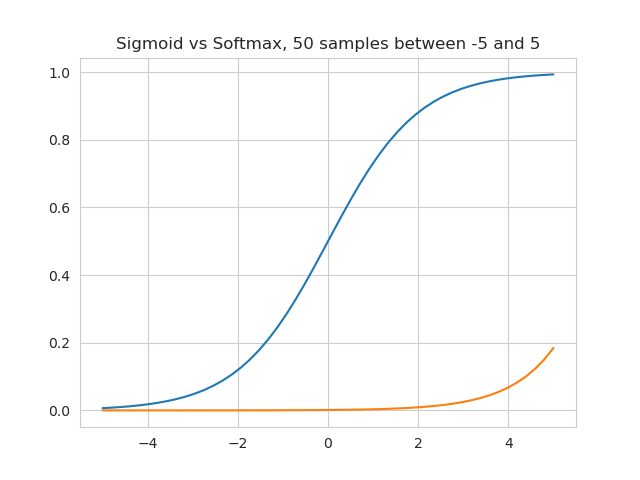
\includegraphics[width=0.6\textwidth]{assets/sigmoid-softmax.png}
  \end{figure}

  Whenever we utilize the softmax activation function, we'll usually use the cross-entropy
  loss function, which is defined as follows:

  \begin{equation*}
    E = - \sum_{i=1}^n z_i \log \hat{z}_i
  \end{equation*}

  The cross-entropy loss function essentially measures the distance between what the
  network thinks the output should be and what it actually is. We utilize it with
  the softmax activation function since our predictions actually represent probabilities
  (i.e they sum to 1).

  Regarding the forward pass, here we can re-utilize every calculation from the previous
  exercise up until activating the last net: here, the activation function is the softmax,
  so we'll have to compute the softmax of the last net.

  \begin{equation*}
    x^{[3]} = \text{softmax}(z^{[3]}) = \begin{bmatrix}
  1 & 1 & 1 & 1\\
\end{bmatrix}
  \end{equation*}

  We'll need, now, to compute the error function's derivative with respect to both
  the weights and the biases. We'll start with the last layer's weights and biases.

  \begin{equation*}
    \begin{aligned}
      \delta^{[3]} & = \frac{\partial E}{\partial z^{[3]}} = \cdots = x^{[3]} - z = \begin{bmatrix}
  0.158216 & 0.205654\\
  -0.815376 & 0.205654\\
  0.158216 & -0.747824\\
\end{bmatrix}                                                       \\
      \delta^{[2]} & = (w^{[3]})^T \delta^{[3]} \circ \text{s'}(z^{[2]}) = \begin{bmatrix}
  0 & 0\\
  0 & 0\\
\end{bmatrix} \circ \text{s'}(z^{[2]}) = \begin{bmatrix}
  -0.0476264 & -0.0283452\\
  -0.0476264 & -0.0283452\\
  -0.0476264 & -0.0283452\\
\end{bmatrix} \\
      \delta^{[1]} & = (w^{[2]})^T \delta^{[2]} \circ \text{s'}(z^{[1]}) = \begin{bmatrix}
  0 & 0\\
  0 & 0\\
\end{bmatrix} \circ \text{s'}(z^{[1]}) = \begin{bmatrix}
  -0.0130754 & -0.00305449\\
  -0.0130754 & -0.00305449\\
  -0.0130754 & -0.00305449\\
  -0.0130754 & -0.00305449\\
\end{bmatrix}
    \end{aligned}
  \end{equation*}

  With $\delta^{[2]}$ and $\delta^{[1]}$ being the zero matrices, both weights and
  biases for their respective layers will not be updated (since the error's derivative
  with respect to them will be 0). Regarding the last layer's weights and biases, though:

  \begin{equation*}
    \begin{aligned}
      \frac{\partial E}{\partial w^{[3]}} & = \delta^{[3]} (x^{[2]})^T = \begin{bmatrix}
  0.124779 & 0.124779 & 0.124779\\
  0.0459927 & 0.0459927 & 0.0459927\\
  -0.170772 & -0.170772 & -0.170772\\
\end{bmatrix}                          \\
      \frac{\partial E}{\partial b^{[3]}} & = \delta^{[3]} \begin{bmatrix}
  1\\
  1\\
\end{bmatrix} = \begin{bmatrix}
  0.36387\\
  -0.609721\\
  -0.589609\\
\end{bmatrix}
    \end{aligned}
  \end{equation*}

  We're now in position to update the weights and biases (these calculations were performed
  for both samples instead of for only the first one, hence the different results
  in comparison with the teacher's solutions):

  \begin{equation*}
    w^{[3]} = \begin{bmatrix}
  0.0796566 & 0.0796566 & 0.0796566\\
  0.100977 & 0.100977 & 0.100977\\
  0.119366 & 0.119366 & 0.119366\\
\end{bmatrix}, \quad
    b^{[3]} = \begin{bmatrix}
  -0.011136\\
  0.0888081\\
  0.0880819\\
\end{bmatrix}
  \end{equation*}

\end{enumerate}

\end{document}